\RequirePackage{color}
\documentclass{ICASP13Paper}

\usepackage{amsmath,amssymb,empheq,amsfonts,amsthm,bm}
\DeclareMathOperator{\E}{\mathbb{E}}
\DeclareMathOperator{\V}{\mathbb{V}}
\newcommand\norm[1]{\left\lVert#1\right\rVert}
\newcommand\fracfun[1]{\textrm{frac}\left(#1\right)}
\DeclarePairedDelimiter\ceil{\lceil}{\rceil}
\DeclarePairedDelimiter\floor{\lfloor}{\rfloor}
\newtheorem{theorem}{Theorem}
%\usepackage{floatrow}


\usepackage{physics}
\usepackage{textcomp}

\usepackage{tikz}
\usepackage{pgfplots}
\usepackage{pgf}
\usepackage{graphicx}
\usepackage{caption}
\usepackage{subcaption}
\usepackage{amssymb}
\usepackage{graphicx}
\usepackage{multirow}
\usepackage{booktabs}
\usepackage{float}



\pgfplotscreateplotcyclelist{my black white}{%
solid, every mark/.append style={solid, fill=gray}, mark=*\\%
dotted, every mark/.append style={solid, fill=gray}, mark=square*\\%
densely dotted, every mark/.append style={solid, fill=gray}, mark=otimes*\\%
loosely dotted, every mark/.append style={solid, fill=gray}, mark=triangle*\\%
dashed, every mark/.append style={solid, fill=gray},mark=diamond*\\%
loosely dashed, every mark/.append style={solid, fill=gray},mark=*\\%
densely dashed, every mark/.append style={solid, fill=gray},mark=square*\\%
dashdotted, every mark/.append style={solid, fill=gray},mark=otimes*\\%
dashdotdotted, every mark/.append style={solid},mark=star\\%
densely dashdotted,every mark/.append style={solid, fill=gray},mark=diamond*\\%
}


% Add an "addauthor" line for each author with the following syntax:
% \addauthor{Name Initials Surname}{Title and affiliation}
\addauthor{Philippe Blondeel}{Graduate Student, Dept. of Computer Science, NUMA Section, KU Leuven, Leuven, Belgium}
\addauthor{Pieterjan Robbe}{Graduate Student, Dept. of Computer Science, NUMA Section, KU Leuven, Leuven, Belgium}
\addauthor{C\'edric Van hoorickx}{Doctor, Dept. of Civil Engineering, KU Leuven, Leuven, Belgium}
\addauthor{Geert Lombaert}{Professor, Dept. of Civil Engineering, KU Leuven, Leuven, Belgium}
\addauthor{Stefan Vandewalle}{Professor, Dept. of Computer Science, NUMA Section, KU Leuven, Leuven, Belgium}

% The title of the abstract
\title{Comparing speed and cost of MLMC with MLQMC in the framework of a practical structural engineering case}

% The bibtex reference file where the references should be found
\referencefile{bib}

% Short abstract of the paper
\shortabstract{\textcolor{red}{The abstract is written last, when the paper is complete. It 
contains a summary of the paper, usually starting with a few words about the 
objectives. Thereafter follow usually statements about the importance of the 
work and the methodology that is employed. The key results are then summarized 
followed by an overview of the conclusions that were drawn from the study.}}

\begin{document}
\section{Introduction}
Models of practical structural engineering applications often exhibit a certain degree of uncertainty. This uncertainty can be located in the dimension of the considered model, the magnitude of the loading forces, material parameters and so forth. In order to address this uncertainty and to quantify it, two main types of methods exist: Non sampling methods and sampling methods. The category of sampling methods encompasses among others the Stochastic Galerkin Finite Element method, see \cite{GhanemAndSpanos}. This method, whilst being highly effective is also highly intrusive and memory demanding due to the transformation of the uncertain coefficient partial differential equation into a large system of coupled of deterministic PDEs by means of a Galerkin projection technique. Sampling methods on the other hand do generally not exhibit this intrusive character. A well known example of such a sampling method is the Monte Carlo (MC) method. For each at random selected sample, the problem is deterministically solved. A major drawback attributed to the Monte Carlo method, is the slow convergence in function of the number of samples taken. This can be however overcome by variance reduction techniques, such as Multilevel Monte Carlo or improved sampling methods, such as Latin Hypercube sampling, see \cite{Loh} or Quasi-Monte Carlo, see \cite{Caflish,Niederreiter}. Multilevel Monte Carlo was first proposed in \cite{Heinrich} and successfully applied in the finance context for option pricing in \cite{Giles}. 

It is in this context that we present our work. Building on the work done in \cite{Blondeel,Blondeel2}, where we compared the speed and cost of Monte Carlo with Multilevel Monte Carlo for a similar structural engineering application and found a speed of a factor ten in favor of Multilevel Monte Carlo, we now combine a Non Linear \textsc{Matlab} Finite Element solver with a \textsc{Julia} Multilevel Monte Carlo and Multilevel Quasi-Monte Carlo implementation by \cite{PJ,PJ2}. Our aim will be to offer a comparison in terms of runtime and cost for a practical structural engineering problem and to demonstrate the versatility  of these two methods. The engineering problem we consider, is defined as a steel beam, clamped at both sides and loaded in the middle where the Young's modulus is considered uncertain.

\section{Case Presentation}
This part introduces the beam characteristics, the modeling of the uncertainty and the Finite Element solver.

\subsection{Beam Characteristics}
In this paper we consider a steel beam clamped on both sides subjected to a static force located in its middle, Fig.\,\ref{fig:bean_configurations}. The beam has the following dimensions and material parameters: $2.5\,\mathrm{m}$ long by $0.25\,\mathrm{m}$ high by $10^{-3}\,\mathrm{m}$ tick, with a yield strength of $240\,\mathrm{MPa}$, a Poisson ratio of $0.25$ and a Young's modulus with a mean value of $200\,\mathrm{GPa}$.


\begin{figure}[h]
\centering
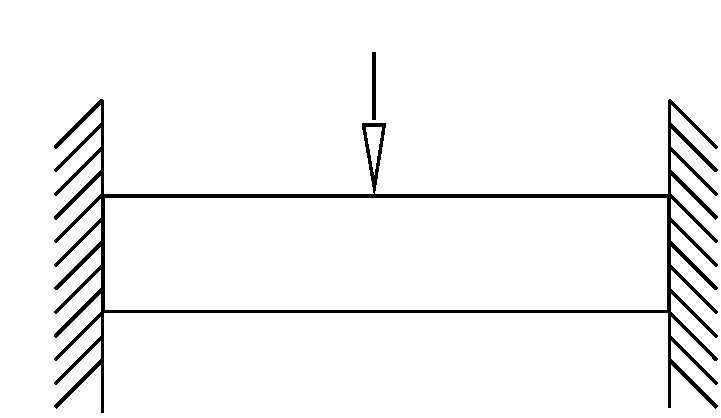
\includegraphics[height=1.9cm]{DoubleClampedBeam.pdf}
\caption{Cantilever beam clamped at both sides loaded in the middle.}
\label{fig:bean_configurations}
\end{figure}

\subsection{Uncertainty Modeling}
The uncertainty resides in the beam's Young's modulus. In order to model this uncertainty, we opt for a heterogeneous representation of it: the uncertainty will be represented by a spatially varying Gamma Random Field constructed by means of a Karhunen-Lo\'eve expansion (KL), see \cite{Loeve}, followed by a memoryless transformation, see \cite{Grigoriu}.

We consider a Gaussian random field $Z\left(\mathbf{x},\omega\right)$, with an exponential covariance kernel,
\begin{equation}
C\left(\mathbf{x},\mathbf{y}\right):=\sigma^2 \exp\left(-\frac{\norm{\mathbf{x}-\mathbf{y}}_1}{\lambda}\right)\,.
\label{eq:covar_kernel}
\end{equation}
The 1-norm is selected together with a correlation length $\lambda = 0.3$ and a standard deviation $\sigma = 1.0$. The KL expansion can then be formulated as follows:
\begin{equation}
Z(\mathbf{x},\omega)=\overline{Z}(\mathbf{x},.)+\sum_{n=1}^{\infty}  \sqrt{\theta_n} \xi_n(\omega) b_n(\mathbf{x})\,.
\end{equation}
The obtained Gaussian random field, $Z(\mathbf{x},\omega)$, is dependent upon respectively the eigenvalues and eigenfunctions, $\theta_n$ and $b_n\left(\mathbf{x}\right)$ of the covariance kernel \eqref{eq:covar_kernel}. $\xi_n\left(\omega\right)$ denotes the i.i.d standard normal random variables. For a one dimensional domain [0,1], the eigenvalue and eigenfunctions can be computed analytically according to 
\begin{equation}
\begin{split}
\label{eq:1D_eigVec}%\label{eq:1D_eigVal}
 &\theta_n^{1\text{D}}= \dfrac{2 \lambda}{\lambda^2 w_n^2 +1}
 ~~~~\mbox{and}~~~ \\
&b^{1\text{D}}_n(x) = A_n \left(\sin(w_n x) +\lambda w_n \cos(w_n x)\right)\,.
\end{split}
\end{equation}
The normalizing constants $A_n$ are chosen such that $ \norm{b_n}_2 = 1$.
The constants $w_n$ represent the real solutions, in increasing order, of the transcendental equation
\begin{equation}\label{eq:transcendental}
\tan(w)=\dfrac{2 \lambda w}{\lambda^2 w^2 -1}\,.
\end{equation}
For the two-dimensional case, the eigenvalues and functions are obtained in a tensorproduct way,
\begin{equation}
\begin{split}
\label{eq:2d_eigenVal}%\label{eq:2d_eigenVec}
&\theta_n^{2\text{D}} = \theta_{i_{n}}^{1\text{D}} \theta_{j_n}^{1\text{D}}
~~~\mbox{and}~~ \\
& b_n^{2\text{D}} (\mathbf{x}) = b_{i_n}^{1\text{D}} (x_1) b_{j_n}^{1\text{D}} (x_2)~~ \mbox{with}~~n = (i_n, j_n)\,.
 \end{split}
\end{equation}

This obtained Gaussian Random field is then transformed to a Gamma Random field by means of a point wise memoryless transformation, see \cite{Grigoriu}. The characteristics of the Gamma distribution are as follows, a shape parameter $\alpha = 934.2$ and a scale parameter $\beta = 0.215 \times 10^{9}$, see \cite{Hess}.

\subsection{Finite Element Modeling}
In order to compute the spatial displacement of the beam in the elasto-plastic region, a Matlab plane stress Finite Element code is used. The beam is discretized by means of an equidistant regular rectangular mesh consisting of four node isoparametric quadrilateral elements. A short overview of the underlying equations and solution methods is presented hereunder.

Due to the nonlinear stress-strain relationship that exists in the elasto-plastic domain, an incremental load approach is used. Starting with a force of $0\,\mathrm{N}$, this force is increased in steps of $135\,\mathrm{N}$ until the total force of $13.5\,\mathrm{kN}$ is reached, for each of these force steps the spatial displacement of the beam is computed by means of a return mapping algorithm. Details about the implementation of this  algorithm can be found in Chapter 2 $\S$4 and Chapter 7 $\S$3 and $\S$4 of \cite{Borst}.

\textcolor{red}{Elaborate a bit?}

\section{Methodology}
This section gives a short overview about the theory pertaining to the Multilevel Monte Carlo method and the Multilevel Quasi-Monte Carlo method. A more detailed analysis can be found in \cite{Giles,Giles2}
\subsection{Multilevel Monte Carlo}
The Multilevel Monte Carlo (MLMC) method is a extension of the standard Monte Carlo (MC) Method, which employs a hierarchy of leveld in order to achieve a variance reduction and by doing so speed up the computation. Here these levels are defined as a hierarchy of nested finite element meshes, Fig.\,\ref{fig:gridrefinement}. The method thus relies on taking many computationally cheap and low resolution samples on coarser meshes and few computationally expensive but high resolution samples on finer meshes.

\begin{figure}
\centering
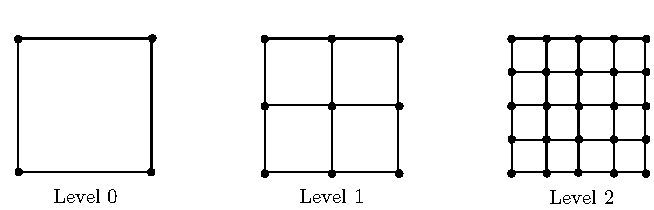
\includegraphics[height=1.9cm]{Grid.pdf}
\caption{Illustrative example of a hierarchy used in the MLMC and MLQMC method.}
\label{fig:gridrefinement}
\end{figure}

The standard MC estimator $Q^{\mathbf{MC}}_{\mathbf{L}}$ for the expected value $\E\left[P_L\right]$ of a particular quantity of interest $P$ using $N_L$ samples is written as
\begin{equation}
Q^{\textrm{MC}}_L={\frac{1}{N_L}}\sum_{n=1}^{N_L} P_L(\omega^n)\,.
\label{eq:MC_est}
\end{equation}
In the case of MLMC, the expected value, $\E\left[P_L\right]$, can be rewritten as follows
\begin{equation}
\E[P_L]=\E[P_0]+\sum_{\ell=1}^L \E[P_\ell -P_{\ell-1}]\,,
\end{equation}
which consequently allows us to write the MLMC as follows
\begin{equation}
\begin{split}
&Q^{\textrm{MLMC}}_L= \frac{1}{N_0}\sum_{n=1}^{N_0} P_0(\omega^{n}) + \\
& \sum_{\ell=1}^L \left \{ \frac{1}{N_\ell} \sum_{n=1}^{N_\ell} \left( P_\ell(\omega^{n})-P_{\ell-1}(\omega^{n})\right) \right \},
\end{split}
\label{eq:MLMC_est}
\end{equation}
Each terms on the right hand side of \eqref{eq:MLMC_est} is estimated separately by a standard MC estimator with $N_\ell$ samples. Compactly the MLMC estimator can be written as a sum of $L + 1 $ estimators for the expected value of the difference on each level, i.e,
\begin{equation}
\begin{split}
&Q^{\textrm{MLMC}}_L = \sum_{\ell = 0}^L Y_{\ell}, \quad \\
& \text{where} \quad Y_{\ell} = \frac{1}{N_\ell} \sum_{n=1}^{N_\ell} \left( P_\ell(\omega^{n})-P_{\ell-1}(\omega^{n})\right).
\end{split}
\end{equation}
with the condition that $P_{-1}\coloneqq0$.
The mean square error (MSE) can be written as follows,
\begin{equation}
\begin{split}
\textrm{MSE}(Q^{\textrm{MLMC}}_L) & := \V\left[Q^{\textrm{MLMC}}_L\right] + \\
&\left(\E\left[Q^{\textrm{MLMC}}_L\right] - \E\left[P\right]\right)^2,
\end{split}
\end{equation}
it encompasses a part pertaining to the variance of the estimator,$\V\left[Q^{\textrm{MLMC}}_L\right]$ and a part pertaining to the squared bias, $\left(\E\left[Q^{\textrm{MLMC}}_L\right] - \E\left[P\right]\right)^2$. The variance of the estimator is computed as
\begin{equation}
\V[Q^{\textrm{MLMC}}_L] = \sum_{\ell=0}^L \frac{V_{\ell}}{N_{\ell}},
\end{equation}
with $V_{\ell}$ denoting the variance of the difference $P_{\ell} - P_{\ell-1}$, will dictate the number of samples needed on each level according to
\begin{equation}\label{eq:nopt}
 N_\ell = \frac{2}{\epsilon^2} \sqrt{\frac{V_\ell}{C_\ell}} \sum_{\ell=0}^L \sqrt{V_\ell C_\ell} .
\end{equation}
MLMC is level adaptive, the decision of adding extra levels lies with the condition on the squared bias, written as $\left(\E[P_{\ell} - P]\right)^2$. The bias can be rewritten as follows. 
\begin{equation}
\abs{\E[P_L-P]} = \abs{\sum_{\ell=L+1}^{\infty} \E[P_\ell-P_{\ell-1}]} \approx \frac{\abs{\E[P_L-P_{L-1}]}}{2^\alpha-1}
\end{equation}
In order for the MSE to be below a given tolerance $\epsilon^2$, the squared bias and the variance of the estimator must both be below $\frac{\epsilon^2}{2}$. Convergence is then checked according to $|\E[P_L-P_{L-1}]|/(2^\alpha-1)\leq\epsilon/\sqrt{2}$ and  $\sum_{\ell=0}^L \frac{V_{\ell}}{N_{\ell}} \leq \frac{\epsilon^2}{2}$.

In the context of this paper and following the approach used in \cite{Blondeel2}, we opt to fix the maximal level for MLMC and MLQMC. This level is defined as level three. The number of elements per level is proportional to $40 \cdot 2^{2 \cdot \ell}$. 

\textcolor{red}{Elaborate over interpretation}

\subsection{Multilevel Quasi-Monte Carlo}
One of the major differences with MLMC is that for Multilevel Quasi-Monte Carlo (MLQMC), the individual sample points are not chosen at random but according to some deterministic rule. Examples of such rules are Sobol\textquotesingle sequences and digital nets. For our application in this paper, we use rank-1 lattice rules as in \cite{Giles3}. These points have the following representation,
\begin{equation}
\mathbf{x}_i = \fracfun{\frac{i}{N}\mathbf{z}},
\label{eq:QMC_points_no_shift}
\end{equation}
where $\fracfun{x}$ stands for the fractional part function which is defined as $\fracfun{x} = x - \floor{x}, x>0$, $\mathrm{z}$ is a $d$-dimensional vector consisting of integers, $n$ being the index and $N$ the number of points.

\begin{figure}
\begin{subfigure}[b]{0.54\linewidth}
\scalebox{0.4}{
% This file was created by matlab2tikz.
%
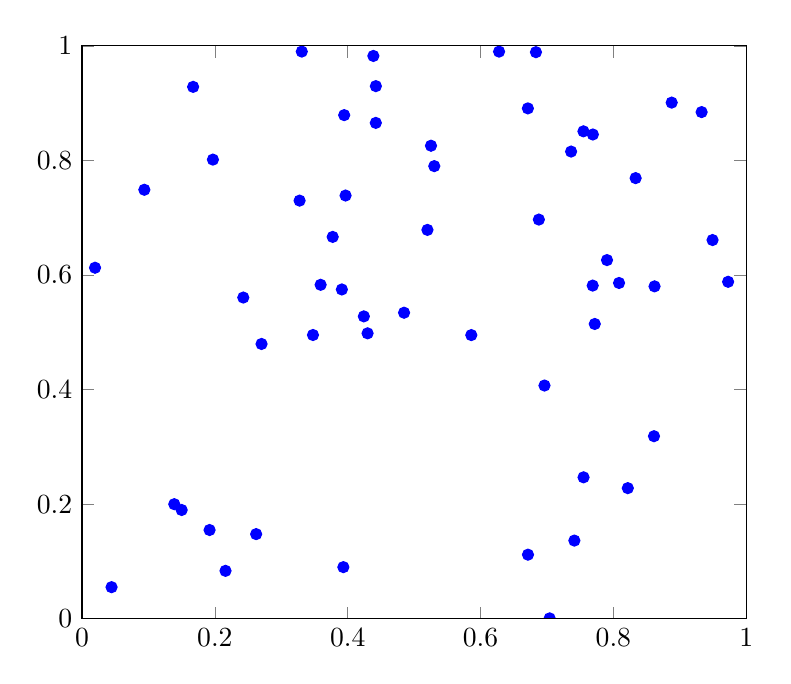
\begin{tikzpicture}
\begin{axis}[%
%width=\figurewidth,
%height=\figureheight,
scale only axis,
xmin=0,
xmax=1,
ymin=0,
ymax=1,
%every tick label/.append style={font=\tiny},
axis background/.style={fill=white},
clip marker paths=true, axis on top=true]
\addplot [color=blue,only marks,mark=*,mark options={solid,fill=blue},forget plot]
  table[row sep=crcr]
  {
0.627896379614169	0.989872153631504 \\
0.771980385554245	0.514423456505704\\
0.93285357027882	0.884281023126955\\
0.972740854003014	0.588026055308497\\
0.192028349427775	0.154752348656045\\
0.138874202829155	0.199862822857452\\
0.696266337082995	0.406954837138907\\
0.0938200267748656	0.748705718215691\\
0.525404403859336	0.825583815786156\\
0.530344218392863	0.789963029944531\\
0.861139811393332	0.318524245398992\\
0.484853333552102	0.534064127370726\\
0.393456361215266	0.089950678770581\\
0.671431139674026	0.111705744193203\\
0.741257943454206	0.136292548938299\\
0.520052467390387	0.678652304800188\\
0.347712671277525	0.495177019089661\\
0.149997253831683	0.18971040601758\\
0.586092067231462	0.495005824990221\\
0.262145317727807	0.147608221976689\\
0.0444540922782385	0.0549741469061882\\
0.754933267231179	0.850712674289007\\
0.242785357820962	0.560559527354885\\
0.442402313001943	0.929608866756663\\
0.687796085120107	0.696667200555228\\
0.359228210401861	0.58279096517584\\
0.736340074301202	0.815397211477421\\
0.394707475278763	0.879013904597178\\
0.683415866967978	0.988911616079589\\
0.704047430334266	0.000522375356944771\\
0.442305413383371	0.865438591013025\\
0.0195776235533187	0.612566469483999\\
0.330857880214071	0.989950205708831\\
0.424309496833137	0.527680069338442\\
0.270270423432065	0.479523385210219\\
0.197053798095456	0.801347605521952\\
0.82172118496131	0.227842935706042\\
0.429921409383266	0.49809429119639\\
0.887770954256354	0.900852488532005\\
0.391182995461163	0.574661219130188\\
0.769114387388296	0.845178185054037\\
0.396791517013617	0.738640291995402\\
0.808514095887345	0.585987035826476\\
0.755077099007084	0.246734525985975\\
0.377395544835103	0.666416217319468\\
0.216018915961394	0.0834828136026227\\
0.790407217966913	0.625959785171583\\
0.949303911849797	0.660944557947342\\
0.327565434075205	0.729751855317221\\
0.67126437045174	0.890752116325322\\
0.438644982586956	0.982303222883606\\
0.833500595588975	0.769029085335896\\
0.768854252429615	0.581446487875398\\
0.167253545494722	0.928313062314188\\
0.861980478702072	0.580090365758442\\
};
\end{axis}
\end{tikzpicture}%
}
\end{subfigure}
\begin{subfigure}[b]{0.45\linewidth}
\scalebox{0.4}{
% This file was created by matlab2tikz.
%
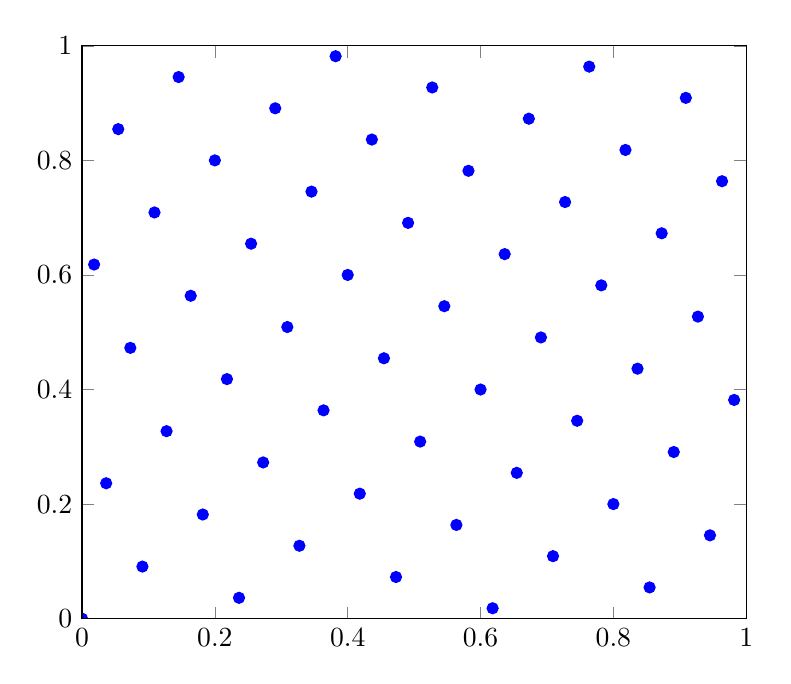
\begin{tikzpicture}


\begin{axis}[%
%width=\figurewidth,
%height=\figureheight,
scale only axis,
xmin=0,
xmax=1,
ymin=0,
ymax=1,
%every tick label/.append style={font=\tiny},
axis background/.style={fill=white},
clip marker paths=true, axis on top=true
]
\addplot [color=blue,only marks,mark=*,mark options={solid,fill=blue},forget plot]
  table[row sep=crcr]
  {%
0	0\\
0.0181818181818182	0.618181818181818\\
0.0363636363636364	0.236363636363636\\
0.0545454545454545	0.854545454545454\\
0.0727272727272727	0.472727272727273\\
0.0909090909090909	0.0909090909090908\\
0.109090909090909	0.709090909090909\\
0.127272727272727	0.327272727272727\\
0.145454545454545	0.945454545454545\\
0.163636363636364	0.563636363636363\\
0.181818181818182	0.181818181818182\\
0.2	0.8\\
0.218181818181818	0.418181818181818\\
0.236363636363636	0.036363636363637\\
0.254545454545455	0.654545454545454\\
0.272727272727273	0.272727272727273\\
0.290909090909091	0.890909090909091\\
0.309090909090909	0.50909090909091\\
0.327272727272727	0.127272727272727\\
0.345454545454545	0.745454545454546\\
0.363636363636364	0.363636363636363\\
0.381818181818182	0.981818181818182\\
0.4	0.6 \\
0.418181818181818	0.218181818181819\\
0.436363636363636	0.836363636363636\\
0.454545454545455	0.454545454545455\\
0.472727272727273	0.0727272727272741\\
0.490909090909091	0.690909090909091\\
0.509090909090909	0.309090909090909\\
0.527272727272727	0.927272727272726\\
0.545454545454545	0.545454545454547\\
0.563636363636364	0.163636363636364\\
0.581818181818182	0.781818181818181\\
0.6	0.399999999999999\\
0.618181818181818	0.0181818181818194\\
0.636363636363636	0.636363636363637\\
0.654545454545455	0.254545454545454\\
0.672727272727273	0.872727272727271\\
0.690909090909091	0.490909090909092\\
0.709090909090909	0.109090909090909\\
0.727272727272727	0.727272727272727\\
0.745454545454545	0.345454545454544\\
0.763636363636364	0.963636363636365\\
0.781818181818182	0.581818181818182\\
0.8	0.199999999999999\\
0.818181818181818	0.818181818181817\\
0.836363636363636	0.436363636363637\\
0.854545454545454	0.0545454545454547\\
0.872727272727273	0.672727272727272\\
0.890909090909091	0.290909090909089\\
0.909090909090909	0.90909090909091\\
0.927272727272727	0.527272727272727\\
0.945454545454545	0.145454545454548\\
0.963636363636364	0.763636363636365\\
0.981818181818182	0.381818181818183\\
};
\end{axis}
\end{tikzpicture}%}
\end{subfigure}
\caption{Example of points sampled for MLMC (left) and MLQMC (right)}
\end{figure}

Due to the deterministic nature of the MLQMC points, a shift has to be introduced in order to be able to obtain unbiased estimates of the quantities of interest. \eqref{eq:QMC_points_no_shift} is rewritten as 
\begin{equation}
\mathbf{x}_n = \fracfun{\frac{n}{N}\mathbf{z} + \Delta},
\end{equation}
where $\Delta$ stands for shift or offset. In practice a number of different random shifts must be chosen $\Delta_1, \Delta_2, ..., \Delta_i$. The MLQMC estimator is then written as 
\begin{equation}
\begin{split}
&Q^{\textrm{MLQMC}}_L= \frac{1}{R_\ell}\sum_{i=1}^{R_\ell}\frac{1}{N_0}\sum_{n=1}^{N_0} P_0(\mathbf{x}_{i,n}) + \\
& \sum_{\ell=1}^L \frac{1}{R_\ell}\sum_{i=1}^{R_\ell}\left \{ \frac{1}{N_\ell} \sum_{n=1}^{N_\ell} \left( P_\ell(\mathbf{x}_{i,n})-P_{\ell-1}(\mathbf{x}_{i,n})\right) \right \}.
\end{split}
\end{equation}
According to good practice, the number of shifts, $R_{\ell}$ in this paper is taken to be 10 on each level. Contrary as for MLMC, the number of samples for MLQMC is not the result of an optimization problem \eqref{eq:nopt}. For MLQMC a doubling algorithm is used as in \cite{Frances}. Starting with a user defined initial number of samples and number of shifts, this doubling algorithm checks the condition on the variance of the system according to $\sum_{l=0}^L V_\ell > \epsilon^2/2$. If the variance is above $\epsilon^2/2$, the number of samples to be taken equals the number already taken times a multiplication constant. In our case this multiplication constant is chosen to be 1.1. 
\subsection{Cost}
Having introduced both methods, we  now present a complexity theorem for MLQMC, which with minor changes is also applicable for MLMC by setting the variable $\delta$ to 1. More details can be found in \cite{Teckentrup}
\begin{theorem}
Given the  positive constants $\alpha, \beta, \gamma, c_1, c_2, c_3$ such that $\alpha \geq \dfrac{1}{2} \mathrm{min}\left(\beta,\delta^{-1}\gamma\right)$ with $\delta \in \left(1/2,1\right]$ and assume that the following conditions hold: 
\begin{enumerate}
\item $\lvert \E[P_{\ell} - P] \rvert \leq c_1 2^{-\alpha \ell}$,
\item $\V\left[Y_{\ell}\right] \leq  c_2 2^{-\beta \ell} N_{\ell}^{-1/\delta} $ \;and
\item $C_{\ell} \leq  c_3 2^{\gamma \ell}$.
\end{enumerate}

Then, there exists a positive constant $c_4$ such that for any $\epsilon < \exp(-1)$ there exists an  $L$ and  a sequence $\{N_{\ell}\}_{\ell=0}^L$ for which the multilevel estimator, $Q^{\mathrm{MLQMC}}_L$ has an $\mathrm{MSE}\leq\epsilon^2$, and
\begin{equation}
\mathrm{cost}(Q^{\mathrm{MLQMC}}) \leq    \left\{
  \begin{aligned}
& c_4 \epsilon^{-2 \delta} && \mathrm{if} \quad  \delta\beta > \gamma, \\
& c_4 \epsilon^{-2 \delta}\left(\log \;\epsilon \right)^{1+\delta} && \mathrm{if} \quad  \delta\beta = \gamma, \\
& c_4 \epsilon^{-2\delta-\left(\gamma-\delta\beta\right)/\alpha} && \mathrm{if} \quad  \delta\beta < \gamma. \\
  \end{aligned}
  \right.
  \label{eq:Algo_regime}
\end{equation}
\label{Theorem_1}
\end{theorem}
Following this theorem, the cost of the MLMC estimator, in its most optimal case  equals $\epsilon^{-2}$. The most optimal cast being defined as when the variance over the levels decreases faster than the cost per level increases, $\beta > \gamma$. Similarly, for the MLQMC estimator, the cost, in the same condition as for MLMC estimator, is proportional to $\epsilon^{-1}$. Note that this is only true in the limit, so the best we can expected is $\delta \approx 1/2$. 

\section{Results}
This section will present a comparison in actual simulation runtime for the considered beam case computed with the MLMC and the MLQMC method. Following this comparison, the variances and the expected values on each level will be shown for each method.  All the results have been computed on a workstation with 14 physical (28 logical cores) Intel Xeon E5-2697 V3, each clocked at $2.6 \,\mathrm{GHz}$, and a total of $128 \,\mathrm{GB}$ RAM.

\subsection{Variances and Expected Values}
This part we validate the results obtained with MLMC and MLQMC by investigating the expected value, the variance, the difference of the expected values and the difference of the variances on each level. Fig.\,\ref{fig:MLMC_var_exp} and Fig.\,\ref{fig:MLQMC_var_exp}, respectively shows this for the MLMC and MLQMC simulation with a tolerance on the RMSE of 2.5E-6.

\begin{figure}[H]
\centering
\begin{subfigure}[b]{0.5\linewidth}
\scalebox{0.5}{
\RequirePackage{luatex85}
\documentclass[tikz]{standalone}
% Default preamble
\usepackage{pgfplots}
\pgfplotsset{compat=newest}
\usepgfplotslibrary{groupplots}
\usepgfplotslibrary{polar}
\usepgfplotslibrary{statistics}
\usepgfplotslibrary{dateplot}
% Custom preamble from global variable:
\usepackage{amsfonts}
\newcommand{\littletriangle}[1]
{
    \pgfplotsextra
    {
        \pgfkeysgetvalue{/pgfplots/xmin}{\xmin}
        \pgfkeysgetvalue{/pgfplots/xmax}{\xmax}
        \pgfkeysgetvalue{/pgfplots/ymin}{\ymin}
        \pgfkeysgetvalue{/pgfplots/ymax}{\ymax}

        \pgfmathsetmacro{\xArel}{0.25}
        \pgfmathsetmacro{\yArel}{0.1}
        \pgfmathsetmacro{\xBrel}{0.1}
        \pgfmathsetmacro{\yBrel}{\yArel}
        \pgfmathsetmacro{\xCrel}{\xBrel}

        \pgfmathsetmacro{\lnxB}{\xmin*(1-(0.1))+\xmax*(0.1)}
        \pgfmathsetmacro{\lnxA}{\xmin*(1-0.25)+\xmax*0.25}
        \pgfmathsetmacro{\lnyA}{\ymin*(1-0.1)+\ymax*0.1}
        \pgfmathsetmacro{\lnyC}{\lnyA+#1*(\lnxA-\lnxB)}
        \pgfmathsetmacro{\yCrel}{\lnyC-\ymin)/(\ymax-\ymin)}
        
        \coordinate (A) at (rel axis cs:\xArel,\yArel);
        \coordinate (B) at (rel axis cs:\xBrel,\yBrel);
        \coordinate (C) at (rel axis cs:\xCrel,\yCrel);

        \draw[black]   (A)--node[pos=0.9,yshift=1ex,xshift=0.5ex] {\small #1}
                    (B)--
                    (C)-- 
                    cycle;
    }
}

\newcommand{\drawsquare}[3]{\draw[thick,black,fill=#3] (#1,#2)--(#1,#2+1)--(#1+1,#2+1)--(#1+1,#2)--cycle;}


\begin{document}
\begin{tikzpicture}
\begin{axis}[ticklabel style={{font=\small}}, major tick length={2pt}, every tick/.style={{black, line cap=round}}, axis on top, legend style={{draw=none, font=\small, at={(0.03,0.03)}, anchor=south west, fill=none, legend cell align=left}}, xlabel={$\ell$}, xtick distance={1}, ylabel={$\log_2(\mathbb{E}[|\;\cdot\;|])$}]
    \addplot[mark={*}, mark size={1pt}, line cap={round}, mark options={solid}, color={red}]
        table[row sep={\\}]
        {
            \\
            0.0  -5.2209187176790985  \\
        }
        ;
    \addlegendentry {$Q_{\ell}$}
    \addplot[mark={*}, mark size={1pt}, line cap={round}, mark options={solid}, color={red}, style={dotted}]
        table[row sep={\\}]
        {
            \\
        }
        ;
    \addlegendentry {$\Delta Q_{\ell}$}
\end{axis}
\end{tikzpicture}
\end{document}
}
\end{subfigure}
\begin{subfigure}[b]{0.5\linewidth}
\scalebox{0.5}{
\RequirePackage{luatex85}
\documentclass[tikz]{standalone}
% Default preamble
\usepackage{pgfplots}
\pgfplotsset{compat=newest}
\usepgfplotslibrary{groupplots}
\usepgfplotslibrary{polar}
\usepgfplotslibrary{statistics}
\usepgfplotslibrary{dateplot}
% Custom preamble from global variable:
\usepackage{amsfonts}
\newcommand{\littletriangle}[1]
{
    \pgfplotsextra
    {
        \pgfkeysgetvalue{/pgfplots/xmin}{\xmin}
        \pgfkeysgetvalue{/pgfplots/xmax}{\xmax}
        \pgfkeysgetvalue{/pgfplots/ymin}{\ymin}
        \pgfkeysgetvalue{/pgfplots/ymax}{\ymax}

        \pgfmathsetmacro{\xArel}{0.25}
        \pgfmathsetmacro{\yArel}{0.1}
        \pgfmathsetmacro{\xBrel}{0.1}
        \pgfmathsetmacro{\yBrel}{\yArel}
        \pgfmathsetmacro{\xCrel}{\xBrel}

        \pgfmathsetmacro{\lnxB}{\xmin*(1-(0.1))+\xmax*(0.1)}
        \pgfmathsetmacro{\lnxA}{\xmin*(1-0.25)+\xmax*0.25}
        \pgfmathsetmacro{\lnyA}{\ymin*(1-0.1)+\ymax*0.1}
        \pgfmathsetmacro{\lnyC}{\lnyA+#1*(\lnxA-\lnxB)}
        \pgfmathsetmacro{\yCrel}{\lnyC-\ymin)/(\ymax-\ymin)}
        
        \coordinate (A) at (rel axis cs:\xArel,\yArel);
        \coordinate (B) at (rel axis cs:\xBrel,\yBrel);
        \coordinate (C) at (rel axis cs:\xCrel,\yCrel);

        \draw[black]   (A)--node[pos=0.9,yshift=1ex,xshift=0.5ex] {\small #1}
                    (B)--
                    (C)-- 
                    cycle;
    }
}

\newcommand{\drawsquare}[3]{\draw[thick,black,fill=#3] (#1,#2)--(#1,#2+1)--(#1+1,#2+1)--(#1+1,#2)--cycle;}


\begin{document}
\begin{tikzpicture}
\begin{axis}[ticklabel style={{font=\small}}, major tick length={2pt}, every tick/.style={{black, line cap=round}}, axis on top, legend style={{draw=none, font=\small, at={(0.03,0.03)}, anchor=south west, fill=none, legend cell align=left}}, xlabel={$\ell$}, xtick distance={1}, ylabel={$\log_2(\mathbb{V}[\;\cdot\;])$}]
    \addplot[mark={*}, mark size={1pt}, line cap={round}, mark options={solid}, color={blue}]
        table[row sep={\\}]
        {
            \\
            0.0  -15.239380633875012  \\
            1.0  -15.255711100000443  \\
            2.0  -15.180917572364262  \\
            3.0  -15.217101605306281  \\
        }
        ;
    \addlegendentry {$Q_{\ell}$}
    \addplot[mark={*}, mark size={1pt}, line cap={round}, mark options={solid}, color={blue}, style={dotted}]
        table[row sep={\\}]
        {
            \\
            1.0  -19.376513503300462  \\
            2.0  -21.963781475594068  \\
            3.0  -24.35127100142315  \\
        }
        ;
    \addlegendentry {$\Delta Q_{\ell}$}
\end{axis}
\end{tikzpicture}
\end{document}
}
\end{subfigure}
\caption{Expected value and variance and their differences over the levels for MLMC for a tolerance of 2.5E-6.}
\label{fig:MLMC_var_exp}
\end{figure}

\begin{figure}[H]
\centering
\begin{subfigure}[b]{0.5\linewidth}
\scalebox{0.5}{
\RequirePackage{luatex85}
\documentclass[tikz]{standalone}
% Default preamble
\usepackage{pgfplots}
\pgfplotsset{compat=newest}
\usepgfplotslibrary{groupplots}
\usepgfplotslibrary{polar}
\usepgfplotslibrary{statistics}
\usepgfplotslibrary{dateplot}
% Custom preamble from global variable:
\usepackage{amsfonts}
\newcommand{\littletriangle}[1]
{
    \pgfplotsextra
    {
        \pgfkeysgetvalue{/pgfplots/xmin}{\xmin}
        \pgfkeysgetvalue{/pgfplots/xmax}{\xmax}
        \pgfkeysgetvalue{/pgfplots/ymin}{\ymin}
        \pgfkeysgetvalue{/pgfplots/ymax}{\ymax}

        \pgfmathsetmacro{\xArel}{0.25}
        \pgfmathsetmacro{\yArel}{0.1}
        \pgfmathsetmacro{\xBrel}{0.1}
        \pgfmathsetmacro{\yBrel}{\yArel}
        \pgfmathsetmacro{\xCrel}{\xBrel}

        \pgfmathsetmacro{\lnxB}{\xmin*(1-(0.1))+\xmax*(0.1)}
        \pgfmathsetmacro{\lnxA}{\xmin*(1-0.25)+\xmax*0.25}
        \pgfmathsetmacro{\lnyA}{\ymin*(1-0.1)+\ymax*0.1}
        \pgfmathsetmacro{\lnyC}{\lnyA+#1*(\lnxA-\lnxB)}
        \pgfmathsetmacro{\yCrel}{\lnyC-\ymin)/(\ymax-\ymin)}
        
        \coordinate (A) at (rel axis cs:\xArel,\yArel);
        \coordinate (B) at (rel axis cs:\xBrel,\yBrel);
        \coordinate (C) at (rel axis cs:\xCrel,\yCrel);

        \draw[black]   (A)--node[pos=0.9,yshift=1ex,xshift=0.5ex] {\small #1}
                    (B)--
                    (C)-- 
                    cycle;
    }
}

\newcommand{\drawsquare}[3]{\draw[thick,black,fill=#3] (#1,#2)--(#1,#2+1)--(#1+1,#2+1)--(#1+1,#2)--cycle;}


\begin{document}
\begin{tikzpicture}
\begin{axis}[ticklabel style={{font=\small}}, major tick length={2pt}, every tick/.style={{black, line cap=round}}, axis on top, legend style={{draw=none, font=\small, at={(0.03,0.03)}, anchor=south west, fill=none, legend cell align=left}}, xlabel={$\ell$}, xtick distance={1}, ylabel={$\log_2(\mathbb{E}[|\;\cdot\;|])$}]
    \addplot[mark={*}, mark size={1pt}, line cap={round}, mark options={solid}, color={red}]
        table[row sep={\\}]
        {
            \\
            0.0  -5.2209187176790985  \\
        }
        ;
    \addlegendentry {$Q_{\ell}$}
    \addplot[mark={*}, mark size={1pt}, line cap={round}, mark options={solid}, color={red}, style={dotted}]
        table[row sep={\\}]
        {
            \\
        }
        ;
    \addlegendentry {$\Delta Q_{\ell}$}
\end{axis}
\end{tikzpicture}
\end{document}
}
\end{subfigure}
\begin{subfigure}[b]{0.5\linewidth}
\scalebox{0.5}{
\RequirePackage{luatex85}
\documentclass[tikz]{standalone}
% Default preamble
\usepackage{pgfplots}
\pgfplotsset{compat=newest}
\usepgfplotslibrary{groupplots}
\usepgfplotslibrary{polar}
\usepgfplotslibrary{statistics}
\usepgfplotslibrary{dateplot}
% Custom preamble from global variable:
\usepackage{amsfonts}
\newcommand{\littletriangle}[1]
{
    \pgfplotsextra
    {
        \pgfkeysgetvalue{/pgfplots/xmin}{\xmin}
        \pgfkeysgetvalue{/pgfplots/xmax}{\xmax}
        \pgfkeysgetvalue{/pgfplots/ymin}{\ymin}
        \pgfkeysgetvalue{/pgfplots/ymax}{\ymax}

        \pgfmathsetmacro{\xArel}{0.25}
        \pgfmathsetmacro{\yArel}{0.1}
        \pgfmathsetmacro{\xBrel}{0.1}
        \pgfmathsetmacro{\yBrel}{\yArel}
        \pgfmathsetmacro{\xCrel}{\xBrel}

        \pgfmathsetmacro{\lnxB}{\xmin*(1-(0.1))+\xmax*(0.1)}
        \pgfmathsetmacro{\lnxA}{\xmin*(1-0.25)+\xmax*0.25}
        \pgfmathsetmacro{\lnyA}{\ymin*(1-0.1)+\ymax*0.1}
        \pgfmathsetmacro{\lnyC}{\lnyA+#1*(\lnxA-\lnxB)}
        \pgfmathsetmacro{\yCrel}{\lnyC-\ymin)/(\ymax-\ymin)}
        
        \coordinate (A) at (rel axis cs:\xArel,\yArel);
        \coordinate (B) at (rel axis cs:\xBrel,\yBrel);
        \coordinate (C) at (rel axis cs:\xCrel,\yCrel);

        \draw[black]   (A)--node[pos=0.9,yshift=1ex,xshift=0.5ex] {\small #1}
                    (B)--
                    (C)-- 
                    cycle;
    }
}

\newcommand{\drawsquare}[3]{\draw[thick,black,fill=#3] (#1,#2)--(#1,#2+1)--(#1+1,#2+1)--(#1+1,#2)--cycle;}


\begin{document}
\begin{tikzpicture}
\begin{axis}[ticklabel style={{font=\small}}, major tick length={2pt}, every tick/.style={{black, line cap=round}}, axis on top, legend style={{draw=none, font=\small, at={(0.03,0.03)}, anchor=south west, fill=none, legend cell align=left}}, xlabel={$\ell$}, xtick distance={1}, ylabel={$\log_2(\mathbb{V}[\;\cdot\;])$}]
    \addplot[mark={*}, mark size={1pt}, line cap={round}, mark options={solid}, color={blue}]
        table[row sep={\\}]
        {
            \\
            0.0  -15.239380633875012  \\
            1.0  -15.255711100000443  \\
            2.0  -15.180917572364262  \\
            3.0  -15.217101605306281  \\
        }
        ;
    \addlegendentry {$Q_{\ell}$}
    \addplot[mark={*}, mark size={1pt}, line cap={round}, mark options={solid}, color={blue}, style={dotted}]
        table[row sep={\\}]
        {
            \\
            1.0  -19.376513503300462  \\
            2.0  -21.963781475594068  \\
            3.0  -24.35127100142315  \\
        }
        ;
    \addlegendentry {$\Delta Q_{\ell}$}
\end{axis}
\end{tikzpicture}
\end{document}
}
\end{subfigure}
\caption{Expected value and variance and their differences over the levels for MLQMC for a tolerance of 2.5E-6.}
\label{fig:MLQMC_var_exp}
\end{figure}

\textcolor{red}{Intoduce the table}

\begin{table}[H]
\caption{Parameters for the MLMC and MLQMC algorithm.}
\centering
  \scalebox{0.75}{
 \begin{tabular}{c c c cc c c}
\toprule
\multirow{3}{*}{RMSE [/]} & \multicolumn{3}{c}{MLMC } & \multicolumn{3}{c}{MLQMC }\\
 \cmidrule(rl{4pt}){2-4}  \cmidrule(rl{4pt}){5-7}
 & $\alpha$ & $\beta$ & $\gamma$ & $\alpha$ & $\beta$ & $\gamma$ \\ [0.5ex]
\cmidrule{1-7}
 2.5E-6 & \textcolor{red}{tbd} & \textcolor{red}{tbd} & \textcolor{red}{tbd} & 1.04 & 1.95 & 0.89 \\
\bottomrule
\end{tabular}}
\label{tab:Parameters for the MLMC  and MLQMC algorithm}
\end{table}

\textcolor{red}{Discus why this decreases, the implications, ect..}

\subsection{Cost Comparison}
Fig.\,\ref{fig:Runtime} compares the actual simulation runtime needed to reach a given tolerance for MLMC and MLQMC. As can be seen the cost order for MLMC is roughly proportional to $\epsilon^{-2}$, while for MLQMC it is proportional to $\epsilon^{-1}$.

\textcolor{red}{Elaborate over cost}
\begin{figure}[H]
\centering
\scalebox{0.65}{



\begin{tikzpicture}[trim axis left,trim axis right]
\begin{axis}[
%width=\figurewidth,
%height=\figureheight,
scale only axis,
xlabel={\small accuracy},
every x tick label/.append style={font=\scriptsize},
every x label/.append style={font=\scriptsize},
ylabel={\small run time},
every y tick label/.append style={font=\scriptsize},
every y label/.append style={font=\scriptsize},
legend style={draw=none,font=\scriptsize,at={(0.03,0.03)},anchor=south west,fill=none, legend cell align={left}},
xmode = log,
 ymode = log]


\addplot [color=red,solid,mark=square*,mark options={solid,fill=red},line width=0.75pt,mark size=1.2,line cap=round, forget plot]
table[]{COmpare/data_MLMC/runtime.txt};

\addplot [color=blue,solid,mark=triangle*,mark options={solid,fill=blue},line width=0.75pt,mark size=1.2,line cap=round, forget plot]
table[]{COmpare/data_MLQMC/runtime.txt};


\end{axis}
\end{tikzpicture}
}
 \caption{\label{fig:time}Total simulation run time in function of RMSE for MLMC \textcolor{red}{$-\blacksquare $} and for MLQMC \textcolor{blue}{$-$\protect\rotatebox[origin=c]{180}{$\blacktriangledown$}}.}
 \label{fig:Runtime}
\end{figure}

Values corresponding to the times shown in Fig.\,\ref{fig:Runtime} are taken up in Tab.\,\ref{table:times}.

\begin{table}[H]
\caption{Actual simulation time in seconds for MLMC and MLQMC.}
\centering
  \scalebox{0.75}{
%  \hspace{-1cm}
 \begin{tabular}{lll}
 \toprule
 \multirow{3}{*}{RMSE [/]} & \multicolumn{2}{c}{Time [sec]}    \\ [0.5ex]  
 % \cmidrule(rl{4pt}){2-3}  
   & MLMC & MLQMC   \\
\cmidrule{1-3}
  9.6E-5 & 1.64E+3 &1.54E+3  \\
  6.4E-5 & 1.65E+3&1.54E+3  \\
  4.2E-5 & 1.65E+3&1.56E+3  \\
  2.8E-5 & 1.67E+3&1.70E+3\\
  1.9E-5 & 2.43E+3& 1.92E+3 \\
  1.2E-5 & 3.58E+3&2.30E+3  \\
  8.4E-6 & 6.79E+3&6.15E+3  \\
  5.6E-6 & 1.52E+4&7.47E+3\\
  3.7E-6 & 4.12E+4&1.61E+4\\
  2.5E-6 & \textcolor{red}{TBD}&2.23E+4\\
  \bottomrule
\end{tabular}}
\label{table:times}
\end{table}

As can be observed from the value in Tab.\,\ref{table:times} and Fig.\,\ref{fig:Runtime}, the simulation time for MLMC and MLQMC is more or less equal up until the tolerance of 1.9E-5. At that time the speedup in favor of MLQMC become apparent. Only for fine enough tolerances will there thus be a speedup. This effect is linked to the sample size needed, indeed for MLQMC, there exists a non-negligible  startup cost. This is because the cost for 1 MLQMC sample is tenfold that of 1 MLMC sample. This is due to the fact that 10 shifts are taken for 1 MLQMC sample. The speedup for MLQMC will thus only become apparent for fine tolerances.

\subsection{Sample sizes}
\textcolor{red}{Show decreasing sample sizes for fines level}
This section presents the sample sizes for the different tolerances for MLMC, Fig.\,\ref{fig:samples_MLMC} and for MLQMC, Fig.\,\ref{fig:samples_MLQMC}.

\begin{figure}[H]
\centering
\scalebox{0.65}{
%!TEX root = ../report_SPDE MC (multiple).tex

\begin{tikzpicture}[trim axis left,trim axis right]
\begin{axis}[
width=\figurewidth,
height=\figureheight,
scale only axis,
xlabel={\small level $\ell$},
every x tick label/.append style={font=\scriptsize},
every x label/.append style={font=\scriptsize},
ylabel={\small number of samples $N_\ell$},
every y tick label/.append style={font=\scriptsize},
every y label/.append style={font=\scriptsize},
legend style={draw=none,font=\scriptsize,at={(0.03,0.03)},anchor=south west,fill=none},
ymode=log,
 xmin=0,
 xmax=0,
 xtick={0,1,...,0},
]


\addplot [color={rgb,1:red,0.0; green,0.0; blue,0.5},solid,mark=*,mark options={solid,fill={rgb,1:red,0.0; green,0.0; blue,0.5}},line width=0.75pt,mark size=1.2]
table[x index = {0}, y index = {1}]{data/samples.txt};


\addplot [color={rgb,1:red,0.0; green,0.0; blue,0.999108734402852},solid,mark=*,mark options={solid,fill={rgb,1:red,0.0; green,0.0; blue,0.999108734402852}},line width=0.75pt,mark size=1.2]
table[x index = {0}, y index = {2}]{data/samples.txt};


\addplot [color={rgb,1:red,0.0; green,0.3784313725490196; blue,1.0},solid,mark=*,mark options={solid,fill={rgb,1:red,0.0; green,0.3784313725490196; blue,1.0}},line width=0.75pt,mark size=1.2]
table[x index = {0}, y index = {3}]{data/samples.txt};


\addplot [color={rgb,1:red,0.0; green,0.8333333333333334; blue,1.0},solid,mark=*,mark options={solid,fill={rgb,1:red,0.0; green,0.8333333333333334; blue,1.0}},line width=0.75pt,mark size=1.2]
table[x index = {0}, y index = {4}]{data/samples.txt};


\addplot [color={rgb,1:red,0.30044275774826057; green,1.0; blue,0.6672991777356103},solid,mark=*,mark options={solid,fill={rgb,1:red,0.30044275774826057; green,1.0; blue,0.6672991777356103}},line width=0.75pt,mark size=1.2]
table[x index = {0}, y index = {5}]{data/samples.txt};


\addplot [color={rgb,1:red,0.6672991777356103; green,1.0; blue,0.30044275774826057},solid,mark=*,mark options={solid,fill={rgb,1:red,0.6672991777356103; green,1.0; blue,0.30044275774826057}},line width=0.75pt,mark size=1.2]
table[x index = {0}, y index = {6}]{data/samples.txt};


\addplot [color={rgb,1:red,1.0; green,0.9012345679012348; blue,0.0},solid,mark=*,mark options={solid,fill={rgb,1:red,1.0; green,0.9012345679012348; blue,0.0}},line width=0.75pt,mark size=1.2]
table[x index = {0}, y index = {7}]{data/samples.txt};


\addplot [color={rgb,1:red,1.0; green,0.48002904865649987; blue,0.0},solid,mark=*,mark options={solid,fill={rgb,1:red,1.0; green,0.48002904865649987; blue,0.0}},line width=0.75pt,mark size=1.2]
table[x index = {0}, y index = {8}]{data/samples.txt};


\addplot [color={rgb,1:red,0.9991087344028523; green,0.07334785766158336; blue,0.0},solid,mark=*,mark options={solid,fill={rgb,1:red,0.9991087344028523; green,0.07334785766158336; blue,0.0}},line width=0.75pt,mark size=1.2]
table[x index = {0}, y index = {9}]{data/samples.txt};


\addplot [color={rgb,1:red,0.5; green,0.0; blue,0.0},solid,mark=*,mark options={solid,fill={rgb,1:red,0.5; green,0.0; blue,0.0}},line width=0.75pt,mark size=1.2]
table[x index = {0}, y index = {10}]{data/samples.txt};


\end{axis}
\end{tikzpicture}
}
 \caption{Total number of samples $N_\ell$ taken on each level for MLMC.}
 \label{fig:samples_MLMC}
\end{figure}

\begin{figure}[h!]
\centering
\scalebox{0.65}{
%!TEX root = ../report_SPDE MC (multiple).tex

\begin{tikzpicture}[trim axis left,trim axis right]
\begin{axis}[
width=\figurewidth,
height=\figureheight,
scale only axis,
xlabel={\small level $\ell$},
every x tick label/.append style={font=\scriptsize},
every x label/.append style={font=\scriptsize},
ylabel={\small number of samples $N_\ell$},
every y tick label/.append style={font=\scriptsize},
every y label/.append style={font=\scriptsize},
legend style={draw=none,font=\scriptsize,at={(0.03,0.03)},anchor=south west,fill=none},
ymode=log,
 xmin=0,
 xmax=0,
 xtick={0,1,...,0},
]


\addplot [color={rgb,1:red,0.0; green,0.0; blue,0.5},solid,mark=*,mark options={solid,fill={rgb,1:red,0.0; green,0.0; blue,0.5}},line width=0.75pt,mark size=1.2]
table[x index = {0}, y index = {1}]{data/samples.txt};


\addplot [color={rgb,1:red,0.0; green,0.0; blue,0.999108734402852},solid,mark=*,mark options={solid,fill={rgb,1:red,0.0; green,0.0; blue,0.999108734402852}},line width=0.75pt,mark size=1.2]
table[x index = {0}, y index = {2}]{data/samples.txt};


\addplot [color={rgb,1:red,0.0; green,0.3784313725490196; blue,1.0},solid,mark=*,mark options={solid,fill={rgb,1:red,0.0; green,0.3784313725490196; blue,1.0}},line width=0.75pt,mark size=1.2]
table[x index = {0}, y index = {3}]{data/samples.txt};


\addplot [color={rgb,1:red,0.0; green,0.8333333333333334; blue,1.0},solid,mark=*,mark options={solid,fill={rgb,1:red,0.0; green,0.8333333333333334; blue,1.0}},line width=0.75pt,mark size=1.2]
table[x index = {0}, y index = {4}]{data/samples.txt};


\addplot [color={rgb,1:red,0.30044275774826057; green,1.0; blue,0.6672991777356103},solid,mark=*,mark options={solid,fill={rgb,1:red,0.30044275774826057; green,1.0; blue,0.6672991777356103}},line width=0.75pt,mark size=1.2]
table[x index = {0}, y index = {5}]{data/samples.txt};


\addplot [color={rgb,1:red,0.6672991777356103; green,1.0; blue,0.30044275774826057},solid,mark=*,mark options={solid,fill={rgb,1:red,0.6672991777356103; green,1.0; blue,0.30044275774826057}},line width=0.75pt,mark size=1.2]
table[x index = {0}, y index = {6}]{data/samples.txt};


\addplot [color={rgb,1:red,1.0; green,0.9012345679012348; blue,0.0},solid,mark=*,mark options={solid,fill={rgb,1:red,1.0; green,0.9012345679012348; blue,0.0}},line width=0.75pt,mark size=1.2]
table[x index = {0}, y index = {7}]{data/samples.txt};


\addplot [color={rgb,1:red,1.0; green,0.48002904865649987; blue,0.0},solid,mark=*,mark options={solid,fill={rgb,1:red,1.0; green,0.48002904865649987; blue,0.0}},line width=0.75pt,mark size=1.2]
table[x index = {0}, y index = {8}]{data/samples.txt};


\addplot [color={rgb,1:red,0.9991087344028523; green,0.07334785766158336; blue,0.0},solid,mark=*,mark options={solid,fill={rgb,1:red,0.9991087344028523; green,0.07334785766158336; blue,0.0}},line width=0.75pt,mark size=1.2]
table[x index = {0}, y index = {9}]{data/samples.txt};


\addplot [color={rgb,1:red,0.5; green,0.0; blue,0.0},solid,mark=*,mark options={solid,fill={rgb,1:red,0.5; green,0.0; blue,0.0}},line width=0.75pt,mark size=1.2]
table[x index = {0}, y index = {10}]{data/samples.txt};


\end{axis}
\end{tikzpicture}
}
 \caption{Total number of samples $N_\ell$ taken on each level for MLQMC.}
 \label{fig:samples_MLQMC}
\end{figure}

Tab.\,\ref{tab:Samples} tables the values corresponding what is presented in Fig.\,\ref{fig:samples_MLMC} and Fig.\,\ref{fig:samples_MLQMC}.

 \begin{table}[H]
 \caption{Number of samples for MLMC and MLQMC.}
 \setlength{\tabcolsep}{.16667em}
\centering
\scalebox{0.75}{
%\hspace{-2cm}
 \begin{tabular}{ccccccccc}
\toprule
% \multirow{5}{*}{RMSE [/]} %
%\cmidrule(rl{4pt}){2-8}   
\multirow{5}{*}{RMSE [/]} & \multicolumn{4}{c}{MLMC} & \multicolumn{4}{c}{MLQMC} \\
\cmidrule(rl{4pt}){2-5} \cmidrule(rl{4pt}){6-9} 
&\multicolumn{4}{c}{level}&\multicolumn{4}{c}{level}\\
\cmidrule(l{8pt}){2-5} \cmidrule(l{8pt}){6-9}
  &{0} & {1} & {2} & {3}  &{0} & {1} &{2} & {3}  \\ [0.5ex]
%\cmidrule{1-15}
  9.6E-5 & 40 & 40 & 40 & 2 &40&40 &40 & 20 \\
  
  6.4E-5 & 40 & 40 & 40 & 2 &40&40& 40 & 20  \\
  
  4.2E-5 & 40 & 40 & 40 & 2 &50&40& 40 & 20  \\
  
  2.8E-5 & 48 & 40 & 40 & 2 & 170&40&40&20  \\
  
  1.9E-5 & 104 & 40 & 40 & 4 & 330 & 50 &40 & 20 \\
  
  1.2E-5 & 222 & 61 & 40 & 6 & 510 & 90 & 40 & 20  \\
  
  8.4E-6 & 1674 & 152 & 60 & 13 & 1150 & 460 & 90 & 30  \\
  
  5.6E-6 & 5790 & 434 & 138 & 40 & 1400 & 410 & 150 & 30  \\
  
  3.7E-6 & 15025 & 1295 & 339 & 113 & 2280 & 700 &330 & 80 \\
  
  2.5E-6 & \textcolor{red}{TBD} & \textcolor{red}{TBD} & \textcolor{red}{TBD} & \textcolor{red}{TBD} & 3050 & 850 & 410 & 130  \\
\bottomrule
\end{tabular}}
\label{tab:Samples}
\end{table}

\section{Conclusion}

\section{REFERENCES}
{\small
\bibliographystyle{ascelike}
\bibliography{\bibfile_Philippe}
}

\end{document}
